\chapter{Balança}
%\setcounter{section}{0}
%%%%%%%%%%%%%%%%%%%%%%%%%%%%%%%%%%%%%%%%%%%%%%%%%%%%%%%%%%%%%%%%
As balanças foram criadas por necessidade durante o desenvolvimento de comercio na antiguidade, os produtos que não recorriam a contagem por unidades, tais como objetos irregulares por exemplo o ouro tinham de se quantificar seu valor, e a forma de medir sua massa tornou-se numa variável de medição para troca de bens.\\
\\
A relíquia mais antiga de uma balança de medir massa foi descoberto na vila de \textit{Indus River}, perto do conhecido por hoje de Pakistão, e estima-se ser por volta de 2000 B.C.\\
Estas primeiras balanças eram alavancas em equilíbrio $[ \; F_{1} \times b_{1c} = F_{2} \times b_{2c} \; ]$, onde nos extremos eram colocados cestos e se colocava os pesos, este estava centrado no seu centro de massa, assim se os pesos nos dois cestos serem iguais fica em equilíbrio (horizontal), era um sistema de comparar com pesos fixos estabelecidos como norma (\textit{contra-pesos}).
\\
\begin{minipage}[!b]{0.45\linewidth}
	\begin{figure}[H]
		\centering
		\includegraphics[height=7cm]{./image/PESTA/general/balanca_1.jpg}
		\caption{Balança medieval}
		\label{balanca_1}
	\end{figure}
\end{minipage}
\hspace{2.2cm}
\begin{minipage}[!b]{0.45\linewidth}
	\begin{figure}[H]
		\centering
		\includegraphics[height=7cm]{./image/PESTA/general/balanca_4.jpg}
		\caption{Balança moderna \cite{book-7}}
		\label{balanca_4}
	\end{figure}
\end{minipage}
\newline
\newline
\newline
Este sistema pode ter uma boa precisão, mas também pode facilmente ser adulterado.
\\
\\
Os métodos de medir a massa de objetos não conheceu nenhumas melhorias tecnológicas relevantes até a era industrial. Só nos fins do século \textit{XVIII} é que o meio de medir a massa de objetos não dependia de \textbf{contra-pesos}. As balanças por molas foi inventado por \textbf{\textit{Richard Salter}}, um fabricante de balanças por volta dos anos de 1770 na Inglaterra.\\
\begin{figure}[H]
	\centering
	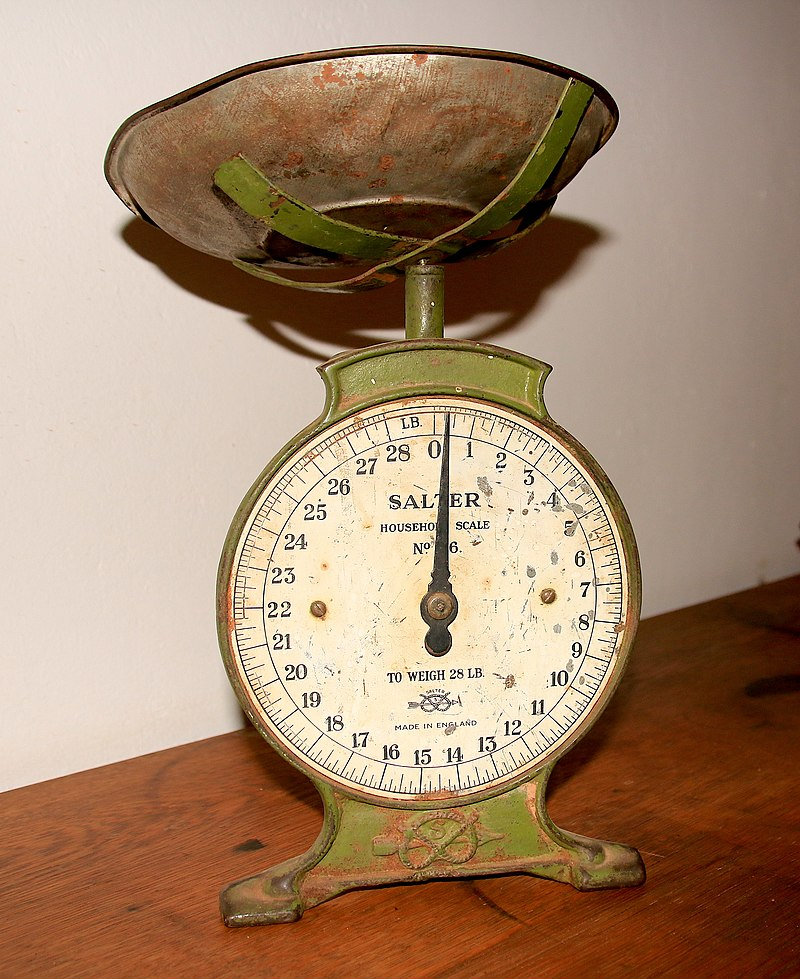
\includegraphics[height=7cm]{./image/PESTA/general/Weigh_Scale_Salter_1.jpg}
	\caption{Balança de Salter}
	\label{Weigh_Scale_Salter_1}
\end{figure}
A balança por mola, como o nome implica, mede a pressão (ou sua tensão) exercido sobre a mola para determinar a massa do objeto. Este tipo de balanças ainda são muito comum nos dias de hoje por serem bastante económicas de fabricar, mas não tem tanta precisão como as eletrónicas desenvolvidas e aperfeiçoadas durante o século \textit{XX}.
\newline
\newline
\begin{minipage}[!b]{\linewidth}
	\begin{figure}[H]
		\captionsetup{justification=raggedright,singlelinecheck=false}
		\flushleft
		\includegraphics[height=7cm]{./image/PESTA/general/Public_Body_Scales_1.jpg}
		\hspace{.8cm}
		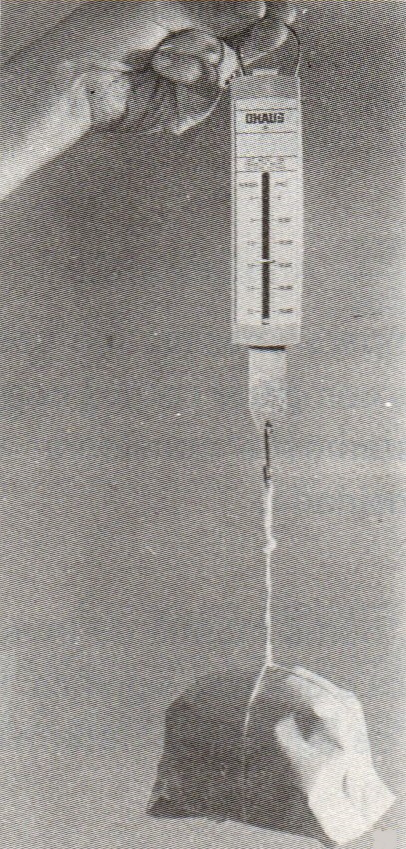
\includegraphics[height=7cm]{./image/PESTA/general/Balanca_Mola_1.jpg}
		\caption{Balanças de Mola}
		\label{Balanca_Mola_1}
	\end{figure}
\end{minipage}
\newpage
As balanças eletrónicas mais modernas utilizam resistências elétricas em materiais permeáveis e fazer passar uma corrente elétrica na qual é possível detetar a variação de condutividade das resistências em que é proporcional a pressão exercida sobre esse material, podendo dai se deduzir o peso dos objetos que se encontrem na balança. \\
\\
O que vai ser utilizado para o projeto vai ser um célula de peso que seque o principio acima mencionado, estes sensores tem quatro \textbf{strain gauges} ligadas em ponte \textit{wheatstone} que vão detetar a distorção do material ou seja a célula de peso e gerar um sinal em tensão proporcional a força exercida. Seque o mesmo principio de uma mola $ [ \; K = \frac{\Delta l}{F} \; ] $.
\\
\\
Também há outros tipos de células de peso tais como as pneumáticas e hidráulicas que convertem a pressão num sinal elétrico que é proporcional a força nela exercida $ [ \; P = \frac{F}{A} \; ] $. As células de peso capacitivas são outro exemplo de como obter um sinal proporcional a força imposta como carga, neste caso é medido sua capacidade pelo afastamento ou aproximação dos pratos dos elétrodos $ [ \; C = \varepsilon_{0} \; \varepsilon_{r} \; \frac{A}{d} \; ] $.
\\
\\
Pode-se dizer que em todos os casos determina-se a força resultante através do deslocamento no espaço.

normaly
